\documentclass[11pt]{article}

\usepackage[margin=1in]{geometry}
\usepackage{graphicx}
\usepackage{booktabs}
\usepackage{xcolor}
\usepackage[colorlinks=true,linkcolor=blue!55!black,urlcolor=blue!55!black]{hyperref}
\usepackage{caption}
\usepackage{float}
\usepackage{enumitem}

\captionsetup{font=small,labelfont=bf}
\setlist{itemsep=2pt,topsep=4pt}
\renewcommand{\arraystretch}{1.15}

\title{\textbf{When the AI Rewrites Its Own History}\\[4pt]
\large Compaction hallucinations, measured across 337 audited summaries}

\author{Johnny Morgan\\ \small University of Maryland, Baltimore County}
\date{\today}

\begin{document}
\maketitle

\begin{abstract}
\noindent
A long AI session eventually runs out of memory. When it does, the model
summarises its own history, discards the original record, and keeps working from
the summary. Everything after that point is built on the summary rather than on
what happened.

We audited 337 of those summaries from 162 sessions by comparing each one against
the full transcript it replaced. The average summary preserved 56\% of what the
session actually contained.

The loss is not uniform, and that is the finding. Git commit hashes survived
99.7\% of the time. What went wrong in the session survived 32\% of the time. The
pattern is a clean gradient: the more a fact is a literal token that either
matches or does not, the better it survives. The more it requires judgement about
what happened, the worse.

One number runs the other way. The measured fabrication rate is zero. The model
does not invent during this step. It loses things and it reshapes things, which
is a different failure and needs a different defence.
\end{abstract}

%======================================================================
\section{What compaction is}

Every AI model has a fixed amount of working memory, called a context window.
A long session fills it. When it fills, something has to give, and what gives is
the detailed history: the model writes a summary of the session so far, the
original messages are dropped, and work continues from the summary.

This is not the model forgetting a fact somebody told it. It is the model
rewriting the record of its own work and then trusting the rewrite. Every
decision after that point rests on the summary being accurate.

\begin{figure}[H]
\centering
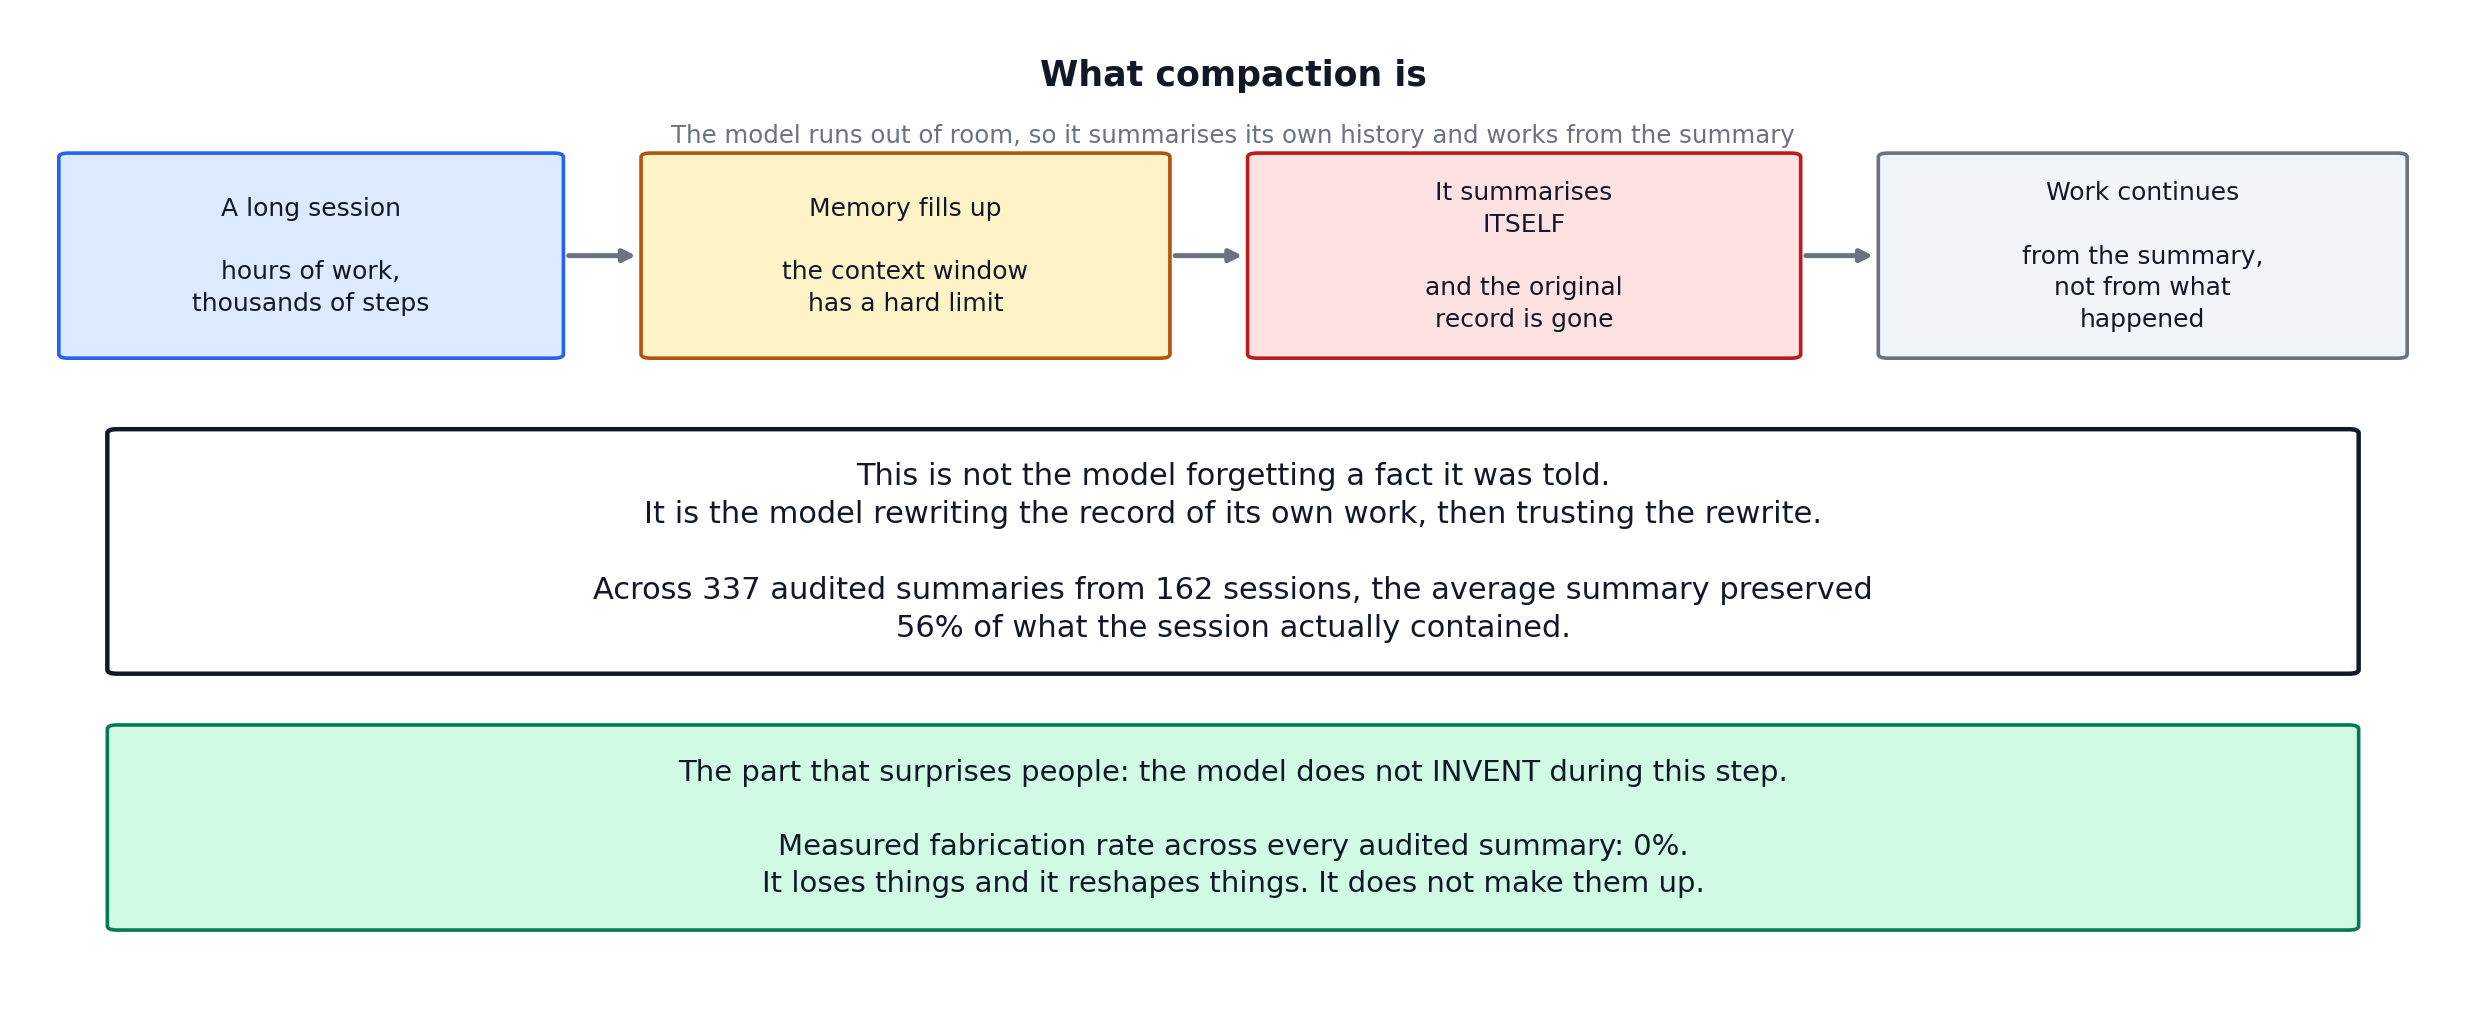
\includegraphics[width=\textwidth]{figures/fig1_what_is_compaction.png}
\caption{The mechanism, and the headline result.}
\end{figure}

\subsection{How it was measured}

For each compaction event we still had the full transcript that the summary
replaced, which makes this checkable rather than a matter of impression. Each
summary was scored against its transcript on seven dimensions plus a fabrication
check: did the commit hashes it cites exist, did the files it names get touched,
did the errors it reports actually occur, is the order of events right, and so
on. Scores are the fraction of the truth the summary preserved.

337 summaries from 162 sessions were audited this way.

%======================================================================
\section{The gradient}

\begin{figure}[H]
\centering
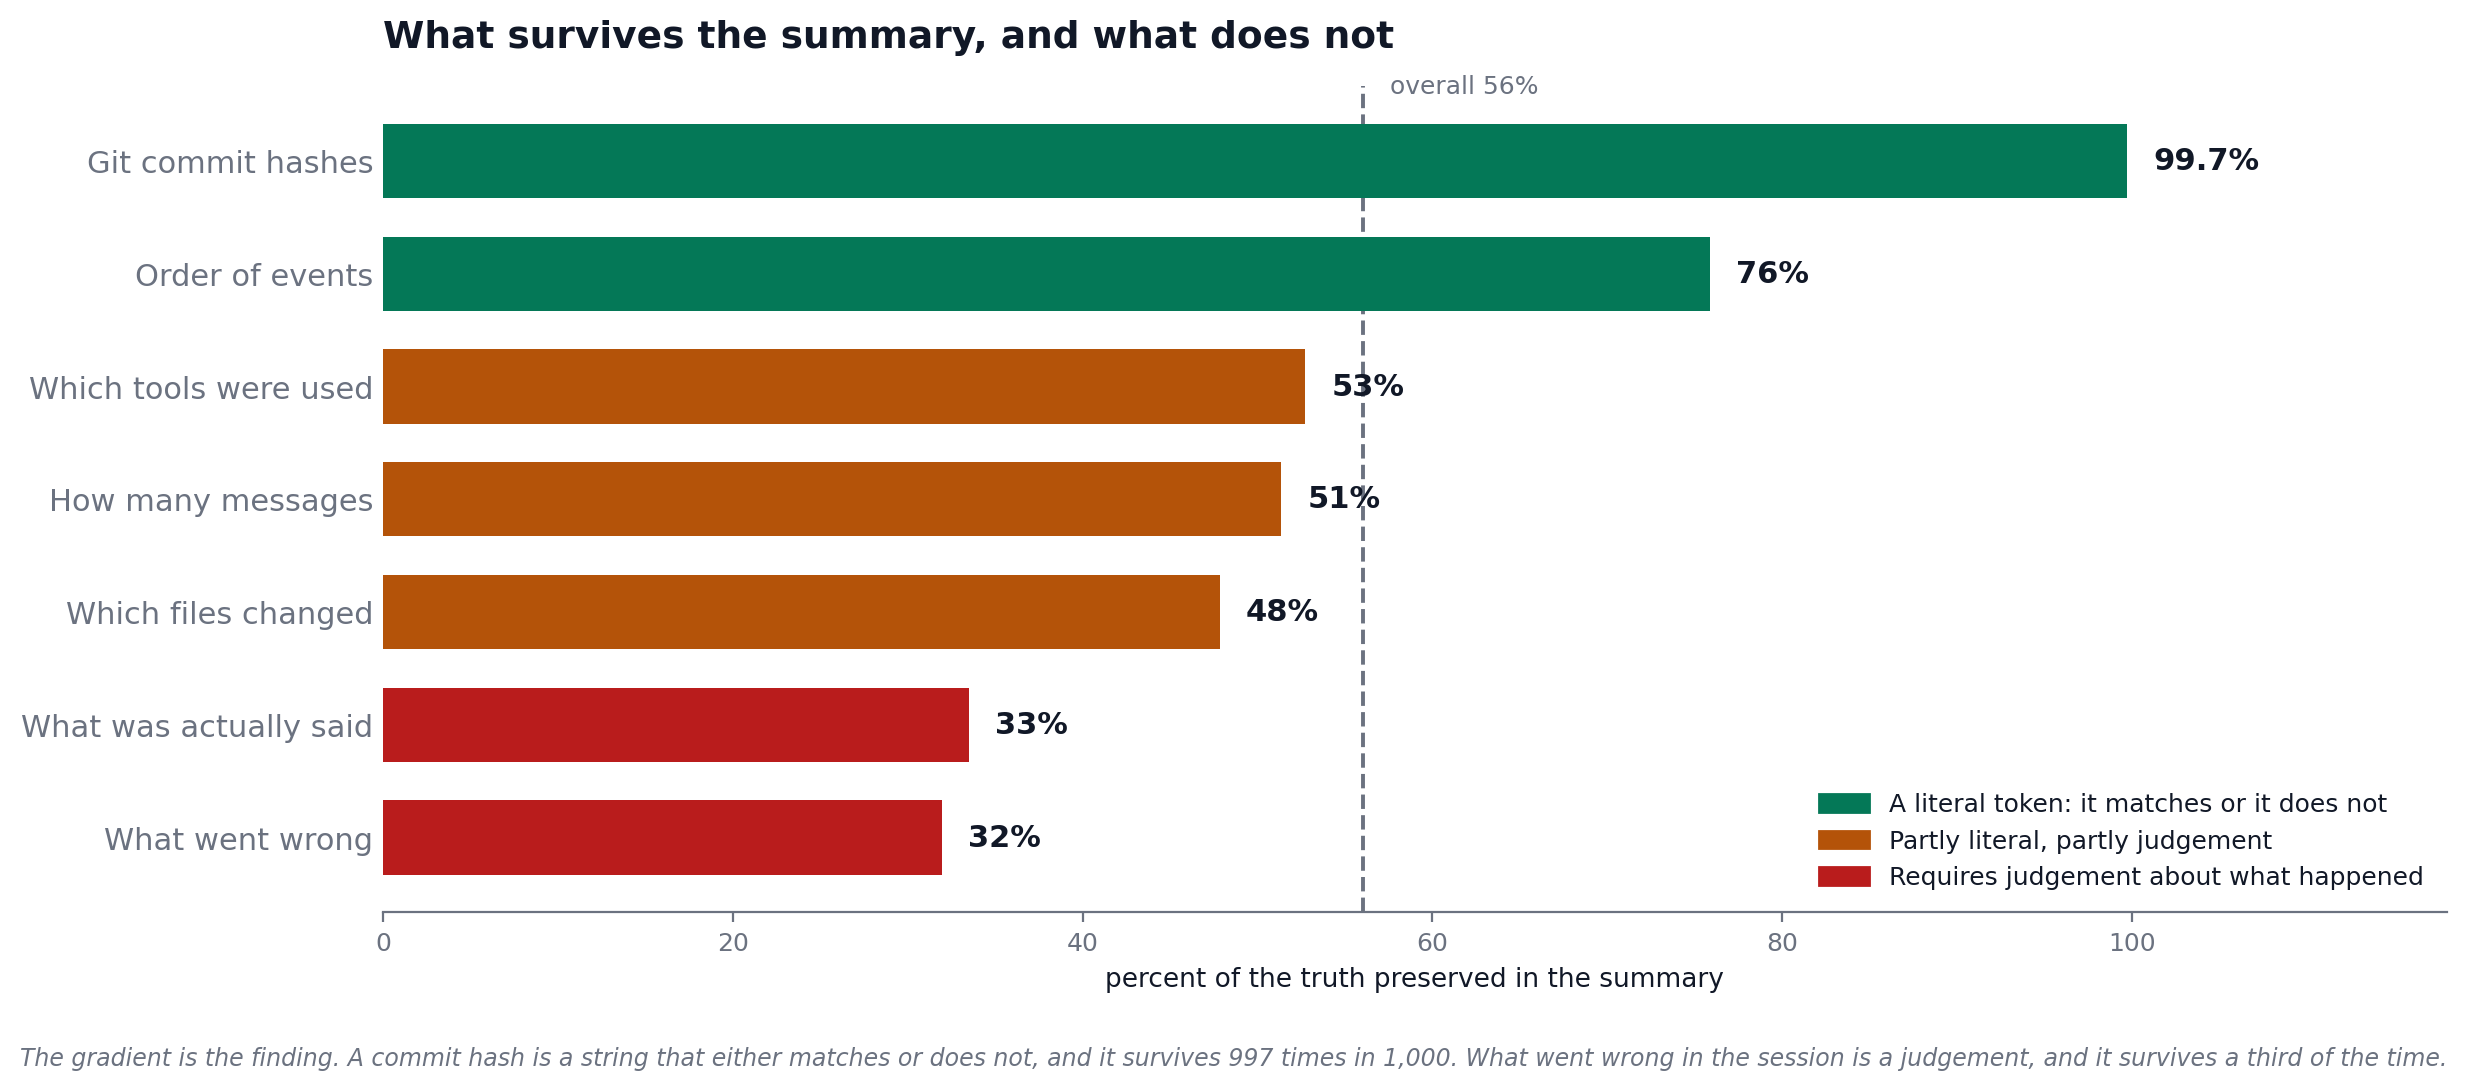
\includegraphics[width=\textwidth]{figures/fig2_fidelity_gradient.png}
\caption{What survives compression and what does not. The ordering is the
result, not a presentation choice.}
\end{figure}

\begin{table}[H]
\centering
\small
\begin{tabular}{lrl}
\toprule
\textbf{What the summary had to preserve} & \textbf{Preserved} & \textbf{Why} \\
\midrule
Git commit hashes        & 99.7\% & A 7-character string. It matches or it does not \\
Order of events          & 75.9\% & Sequence, mostly mechanical \\
Which tools were used     & 52.7\% & Partly a list, partly a judgement of relevance \\
How many messages         & 51.4\% & A count, but of things worth mentioning \\
Which files changed       & 47.8\% & A list, filtered by what seemed important \\
What was actually said    & 33.5\% & Requires representing meaning, not tokens \\
What went wrong           & 31.9\% & Requires deciding what counted as going wrong \\
\midrule
Fabrication rate          & 0.0\%  & Nothing invented, in any summary \\
\midrule
\textbf{Overall}          & \textbf{56.1\%} & weighted across the seven dimensions \\
\bottomrule
\end{tabular}
\caption{The gradient runs from literal tokens at the top to interpretive
judgements at the bottom.}
\end{table}

The interpretation is straightforward. A commit hash is a symbol. Copying it
correctly requires no understanding, and it is either right or wrong, so it
survives compression almost perfectly. ``What went wrong in this session''
requires deciding what counted as an error, how serious it was, and whether it
was resolved. That is interpretation, and interpretation is what compression
destroys.

The practical consequence: after a compaction, the model is most reliable about
exactly the things you could have looked up yourself, and least reliable about
the things you would actually ask it.

%======================================================================
\section{How much simply disappears}

\begin{figure}[H]
\centering
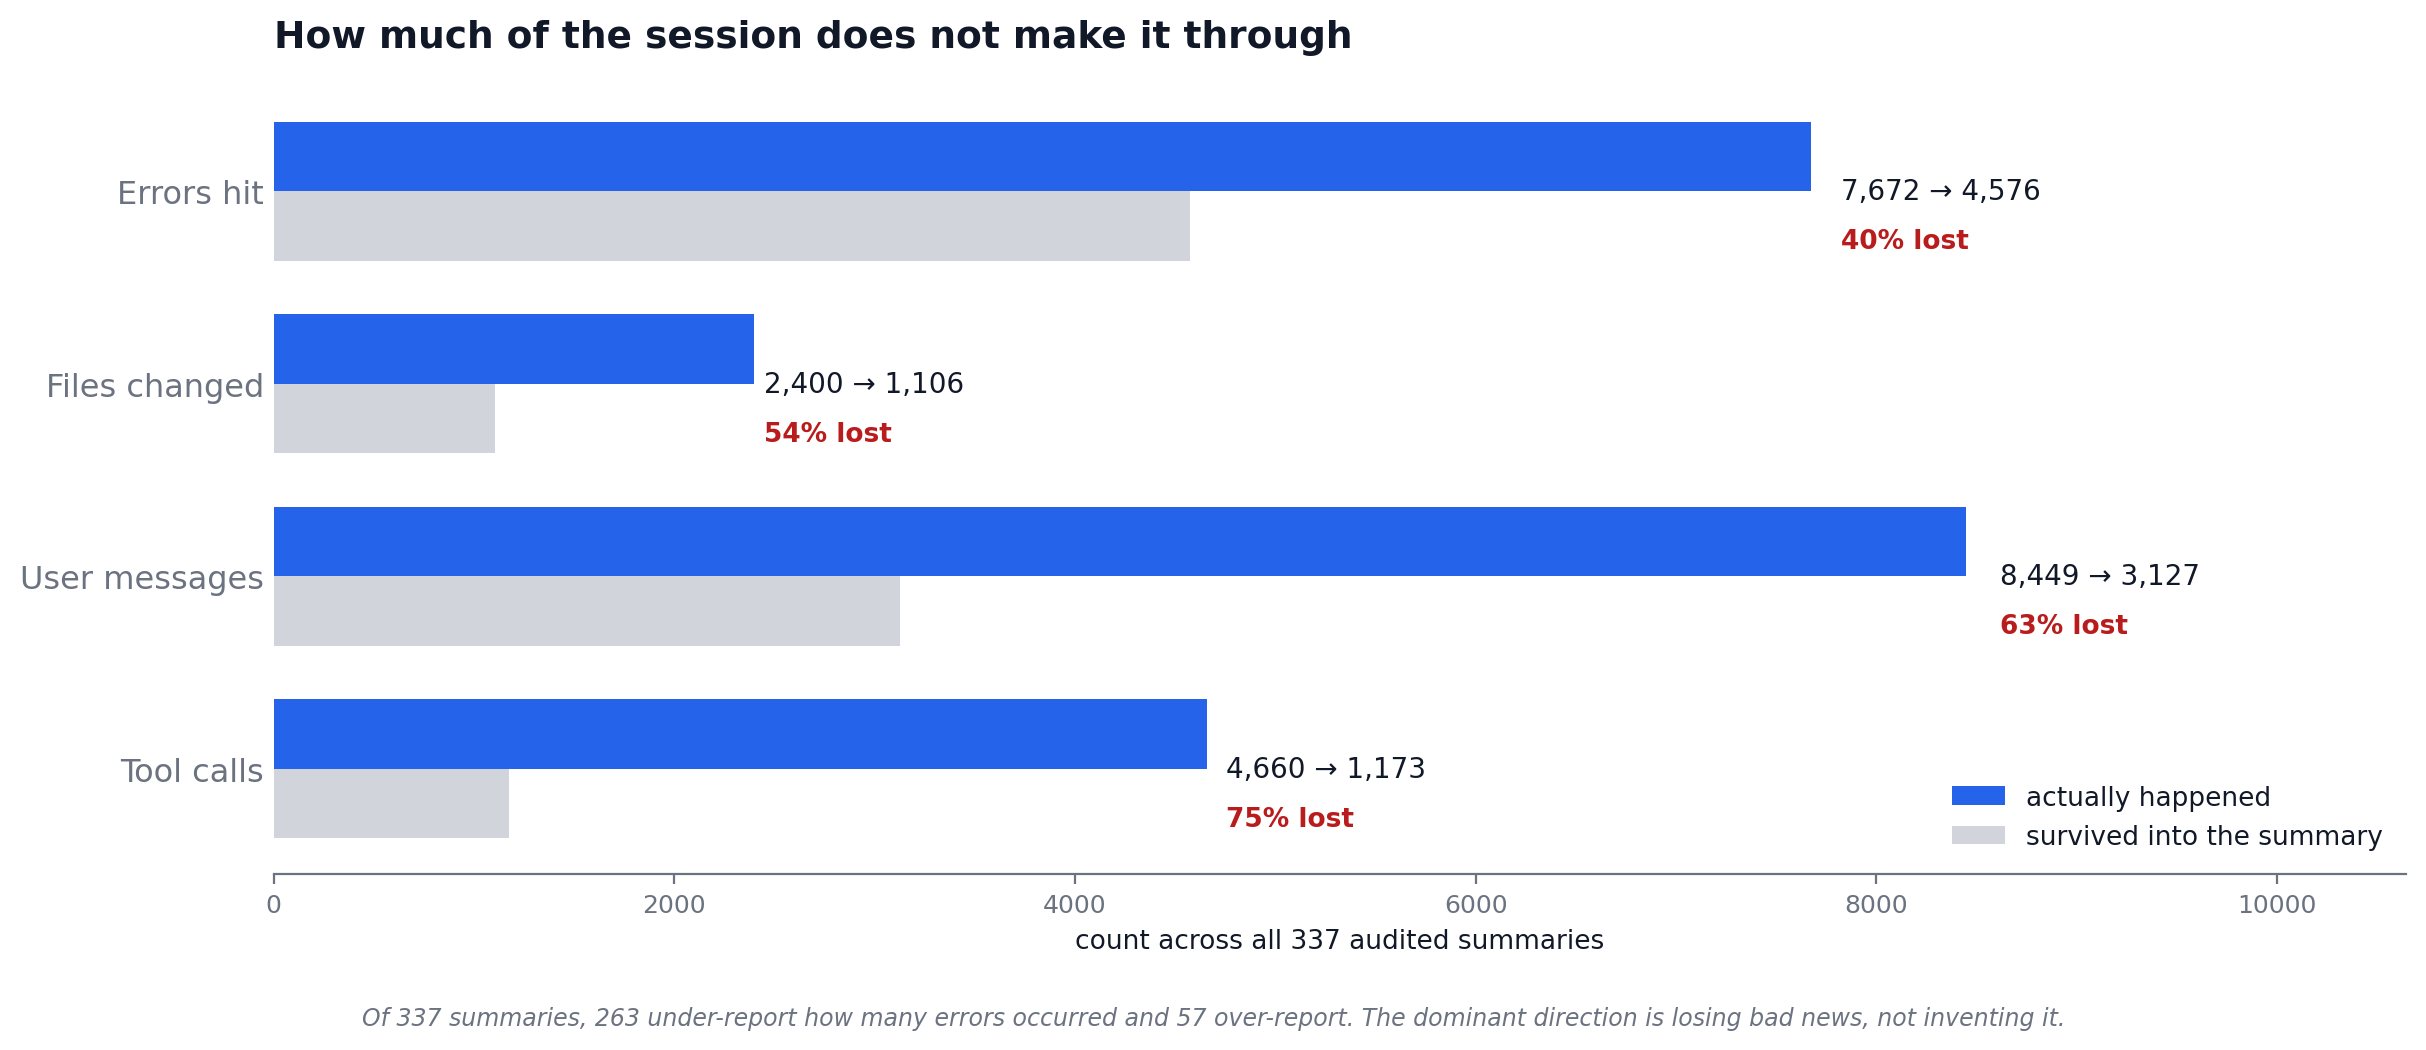
\includegraphics[width=\textwidth]{figures/fig3_what_gets_dropped.png}
\caption{Totals across all 337 audited summaries.}
\end{figure}

\begin{table}[H]
\centering
\small
\begin{tabular}{lrrr}
\toprule
& \textbf{Happened} & \textbf{Survived} & \textbf{Lost} \\
\midrule
Tool calls     & 4{,}660 & 1{,}173 & 75\% \\
User messages  & 8{,}449 & 3{,}127 & 63\% \\
Files changed  & 2{,}400 & 1{,}106 & 54\% \\
Errors hit     & 7{,}672 & 4{,}576 & 40\% \\
\bottomrule
\end{tabular}
\caption{What reached the summary, in aggregate.}
\end{table}

Two observations worth separating.

\textbf{The direction is loss, not invention.} Of 337 summaries, 263 report
fewer errors than actually occurred and 57 report more. Combined with a zero
fabrication rate, the picture is a model that drops bad news rather than
manufacturing it. That matters for what defence you build: a fact-checker aimed
at invented claims would find almost nothing here.

\textbf{Most of the damage carries no warning label.} We tag four specific
compaction pathologies: narrative smoothing, error inflation, compression
artifacts, and message dropping. 207 of the 337 summaries, 61\%, carry no tag at
all, and their mean fidelity is 55.5\%, essentially the same as the tagged ones.
The tags catch specific recognisable distortions. The broader loss is diffuse
and silent, and no flag fires on it.

%======================================================================
\section{Did anything reduce it?}

Partway through this window, a working practice changed. Instead of letting
sessions run until the model was forced to compact, the human began deliberately
ending sessions first and starting fresh, a habit that came to be called
``landing the plane''. It began on 14 February 2026 and appears 202 times in the
record.

\begin{figure}[H]
\centering
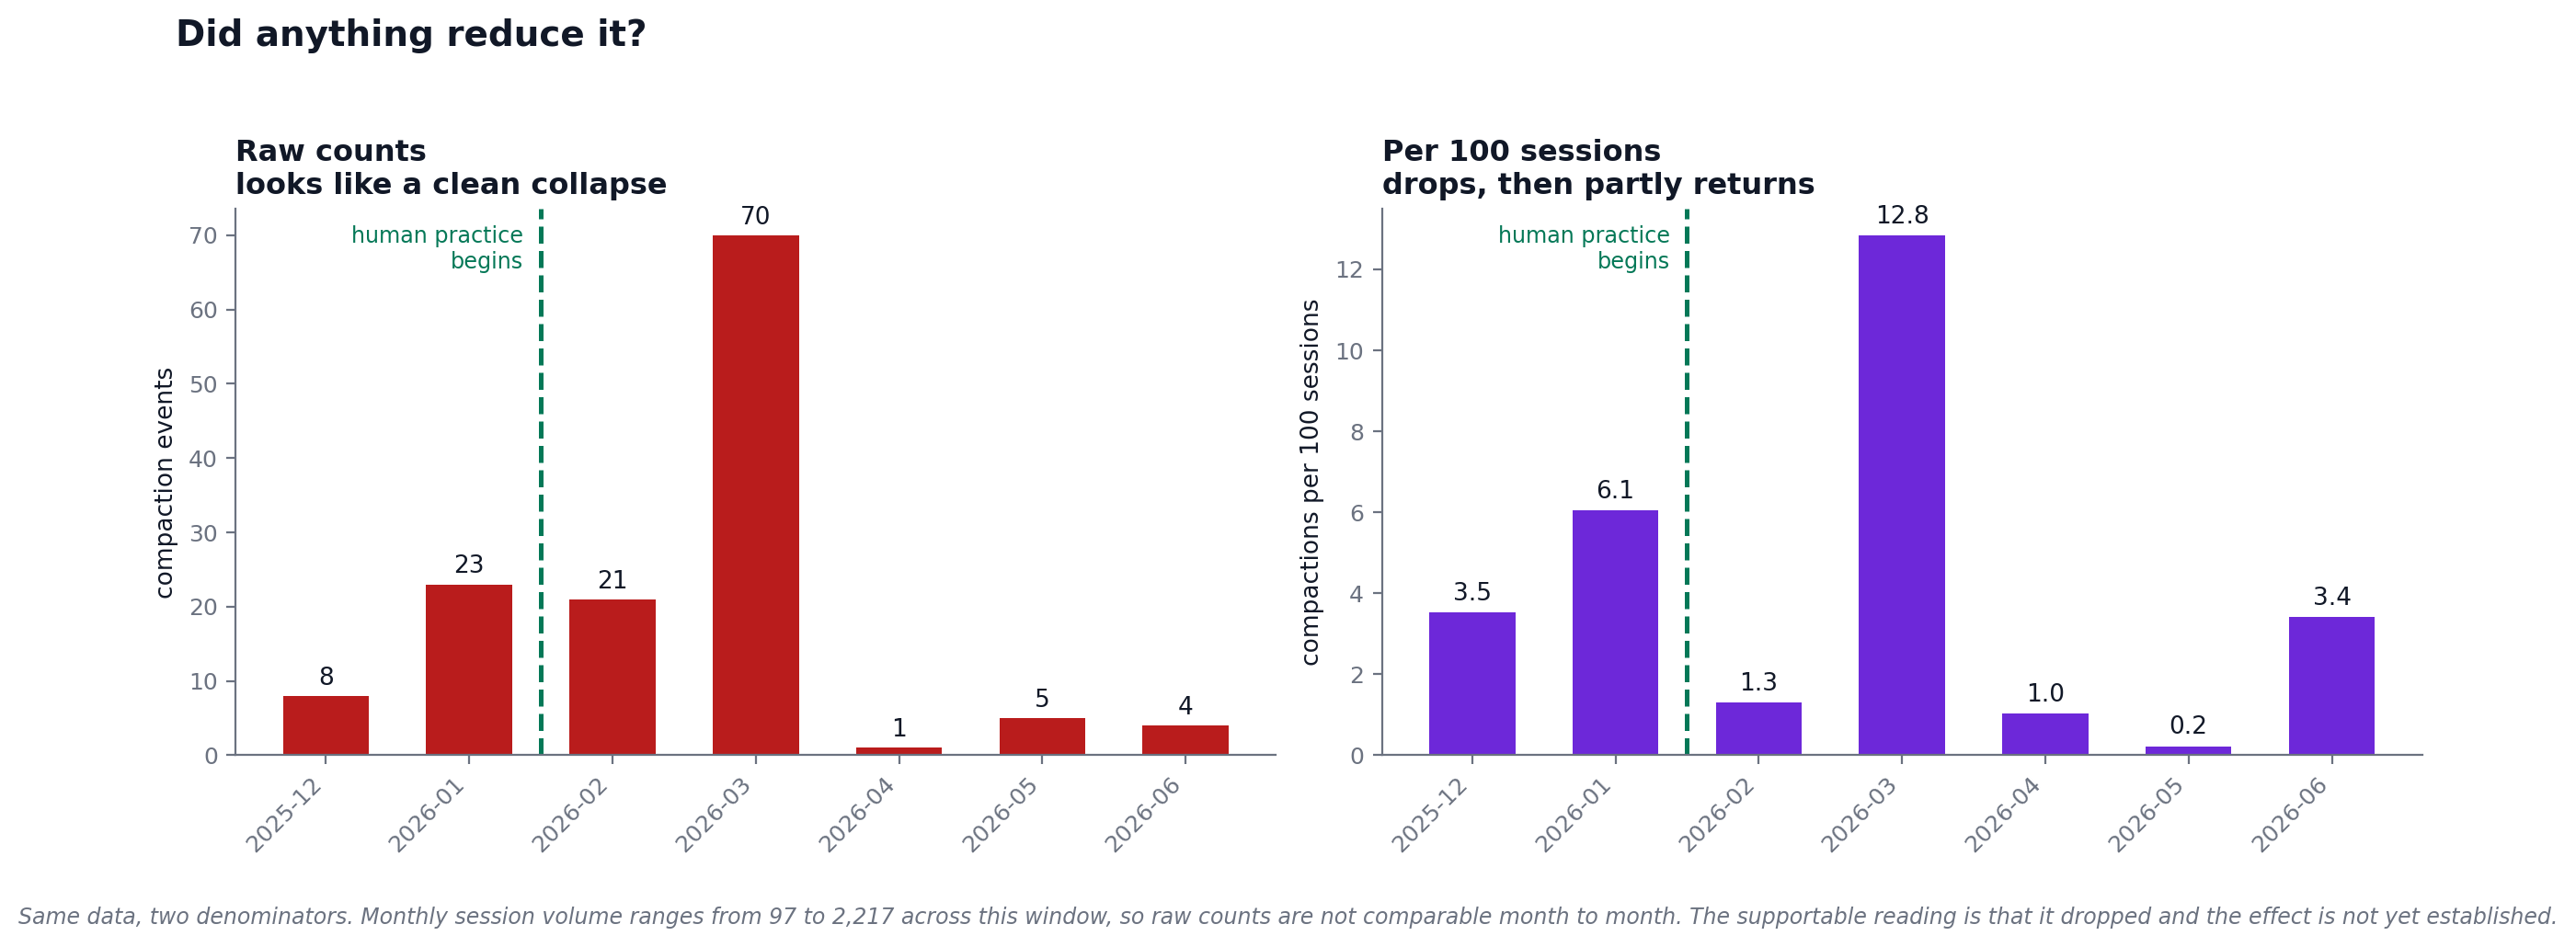
\includegraphics[width=\textwidth]{figures/fig4_intervention.png}
\caption{The same data under two denominators. The left panel is what a slide
deck usually shows. The right panel is what the left panel omits.}
\end{figure}

The raw counts look decisive: compaction events peak at 70 in March and fall to
1 in April.

They are also not comparable month to month. Session volume over this window
ranges from 97 in April to 2,217 in May, a swing of more than 20 times. Once
normalised to compactions per 100 sessions, the March peak is still there at
12.8 and April still falls to 1.0, but June returns to 3.4, which is roughly
where December sat at 3.5, before the practice existed.

So the supportable statement is narrow: compaction became less frequent after the
practice began, and the effect is not established. Nothing here rules out the
alternative that sessions simply got shorter for unrelated reasons, or that the
March spike was itself the anomaly. A matched comparison is open work.

We state this in detail because a briefing that showed only the left panel would
have committed the same error the taxonomy exists to catch: a confident claim
that the underlying record does not support.

%======================================================================
\section{What this means in practice}

\textbf{Treat a post-compaction summary as a lead, not a record.} It is reliable
about identifiers and unreliable about interpretation. If a decision depends on
what went wrong earlier, go back to the source rather than asking the model to
recall it.

\textbf{Anything that must survive should be written as a symbol.} Commit hashes
survived at 99.7\% because they are literal strings with no interpretation in the
middle. The same property is available to anyone designing what a system records:
file paths, identifiers, and exact error text survive compression in a way that
prose summaries do not.

\textbf{End long sessions deliberately.} Whether or not the effect here is
established, a session that ends before it is forced to compact never produces a
compaction hallucination at all. The cheapest defence against a lossy step is
avoiding the step.

\textbf{Do not build the defence around fabrication.} Zero invented content
across 337 summaries. The failure is omission and distortion, and a checker
looking for made-up facts would pass every one of these summaries while the
session record quietly degraded.

%======================================================================
\section{What this does not show}

\textbf{One project, one system.} These are research engineering sessions with
one assistant. The mechanism is general to any system that compresses its own
context, but the numbers are local.

\textbf{The audit is automated.} Fidelity scores come from programmatic
comparison of summary claims against the transcript. That is repeatable and it is
narrower than a human reading would be. A summary can score well by naming the
right things while still misleading about their significance.

\textbf{Counts are a floor.} These are the compaction events we detected. The
audited corpus has its own cutoff, which is a property of the corpus rather than
of when compaction stopped happening.

\textbf{The intervention analysis is correlational.} Stated above and repeated
here because it is the claim most likely to be quoted without its caveat.

%======================================================================
\section{Where a deeper discussion would go}

\begin{enumerate}
  \item \textbf{Can the summary be constrained?} If literal tokens survive and
        interpretation does not, a summary format that forces exact identifiers
        rather than prose should measurably raise fidelity. That is testable
        against the same audit.
  \item \textbf{What happens across repeated compactions?} A session that
        compacts twice is working from a summary of a summary. Whether loss
        compounds linearly or faster is unmeasured here.
  \item \textbf{Does the model know it lost something?} Nothing in these
        summaries flags uncertainty about the parts that were dropped.
  \item \textbf{Is the intervention real?} A matched comparison against sessions
        that did not adopt the practice would settle the correlational question
        in Section 4.
\end{enumerate}

\end{document}
